\newpage
    
\chapter{Partie II : Matériel et Expérimentation}

La mise en œuvre pratique du docking autonome nécessite une intégration matérielle rigoureuse et une validation progressive. Cette partie décrit la plateforme robotique, le capteur principal, ainsi que les deux phases expérimentales menées pour valider nos algorithmes.

\section{Plateforme Robotique : BlueROV Heavy}

Dans cette section, nous présentons le matériel utilisé pour la réalisation de notre projet de docking via notre BlueROV.

Nous présenterons ses spécificités techniques dans les grandes lignes, étant donné que nous n'avons pas modifié le matériel, ni l'électronique du BlueROV.


\subsection{Matériel}

\begin{figure}[h!]
    \centering
    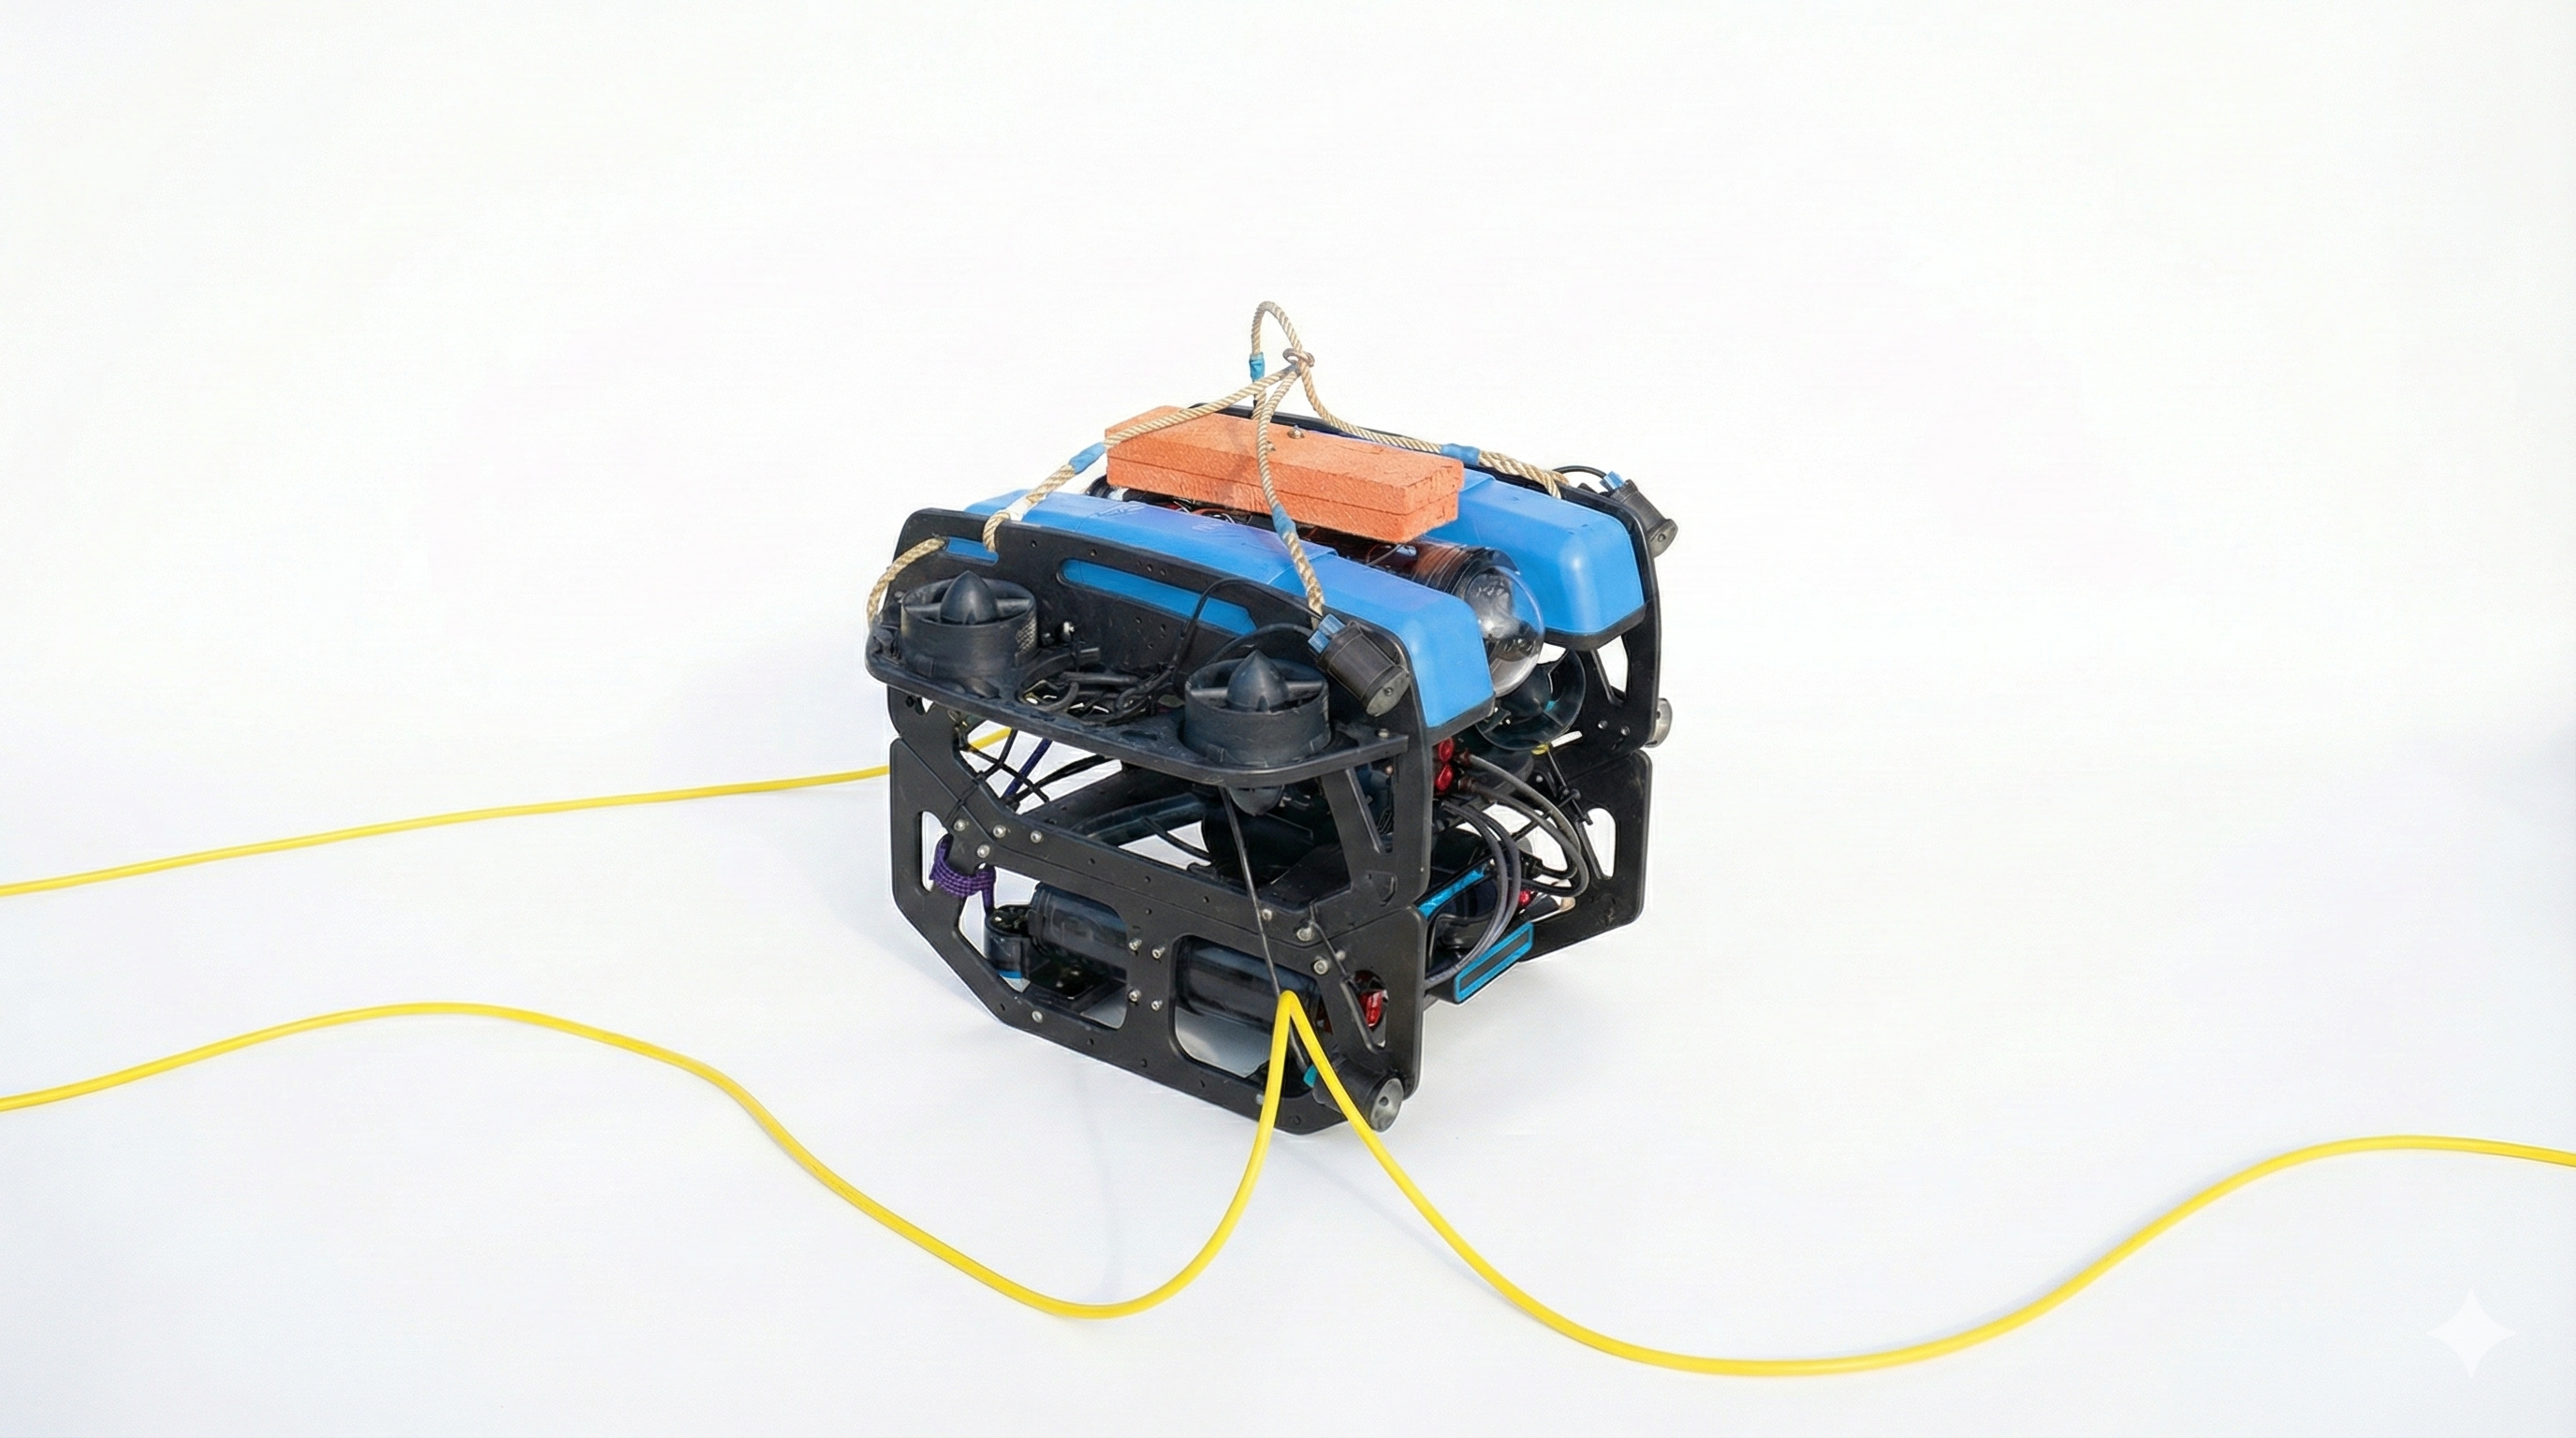
\includegraphics[width=\textwidth]{images/BlueROV.png}
    \caption{Illustration de notre BlueROV}
    \label{fig:bluerov_materiel} % Ensure this label is defined
\end{figure}

La figure \ref{fig:bluerov_materiel} montre le BlueROV utilisé pour le projet de docking autonome.


Pour la perception et le docking, le ROV embarque le sonar multifaisceaux Oculus M750d (Blueprint Subsea). Exploité sur la bande de fréquence ..., il offre la résolution nécessaire aux manœuvres fines : 2.5~mm en portée et $0.6^{\circ}$ en azimut. Il possède une portée allant jusqu'à 120~m. La communication et l'alimentation du ROV est assuré par un tether. Le robot est alimenté par deux Batterie Lipo 4S 14,8V, offrant une autonomie d'environ 2 heures en utilisation normale. L'architecture propulsive du BlueROV Heavy, articulée autour de huit propulseurs (quatre horizontaux et quatre verticaux), confère au véhicule un caractère holonome complet. En effet, cette configuration vectorielle permet de commander indépendamment et simultanément les six degrés de liberté : les trois translations et les trois rotations (lacet, roulis, tangage). Cette omnidirectionnalité garantit une manœuvrabilité fine, permettant au ROV d'effectuer des déplacements latéraux ou verticaux tout en conservant une orientation angulaire fixe, une caractéristique indispensable pour la précision des manœuvres effectuées. Des morceaux de mousses syntactiques sont fixés sur le ROV pour affiner la flottabilité.


\subsection{Conception et Évolution de la Cage de Docking}
\label{sec:cage_materiel}

La conception de la cage a fait l'objet d'un processus itératif combinant tests en bassin et optimisation de la signature acoustique. Cette section détaille l'évolution du prototype initial jusqu'à la configuration finale retenue.

\subsubsection*{Prototype initial : structure simple en PVC}

Les premiers essais ont été menés avec une structure minimale représentant uniquement l'entrée de la cage (figure~\ref{fig:cage}). Cette "porte" en PVC, pourvue de réflecteurs en mousses, présentait une signature acoustique fintéressante, rendant la détection réalisable à quelques mètres. Cependant, la ponctualité des échos et l'absence de repères distincts rendaient l'estimation de l'orientation instable, limitant la fiabilité du guidage.

\begin{figure}[H]
    \centering
    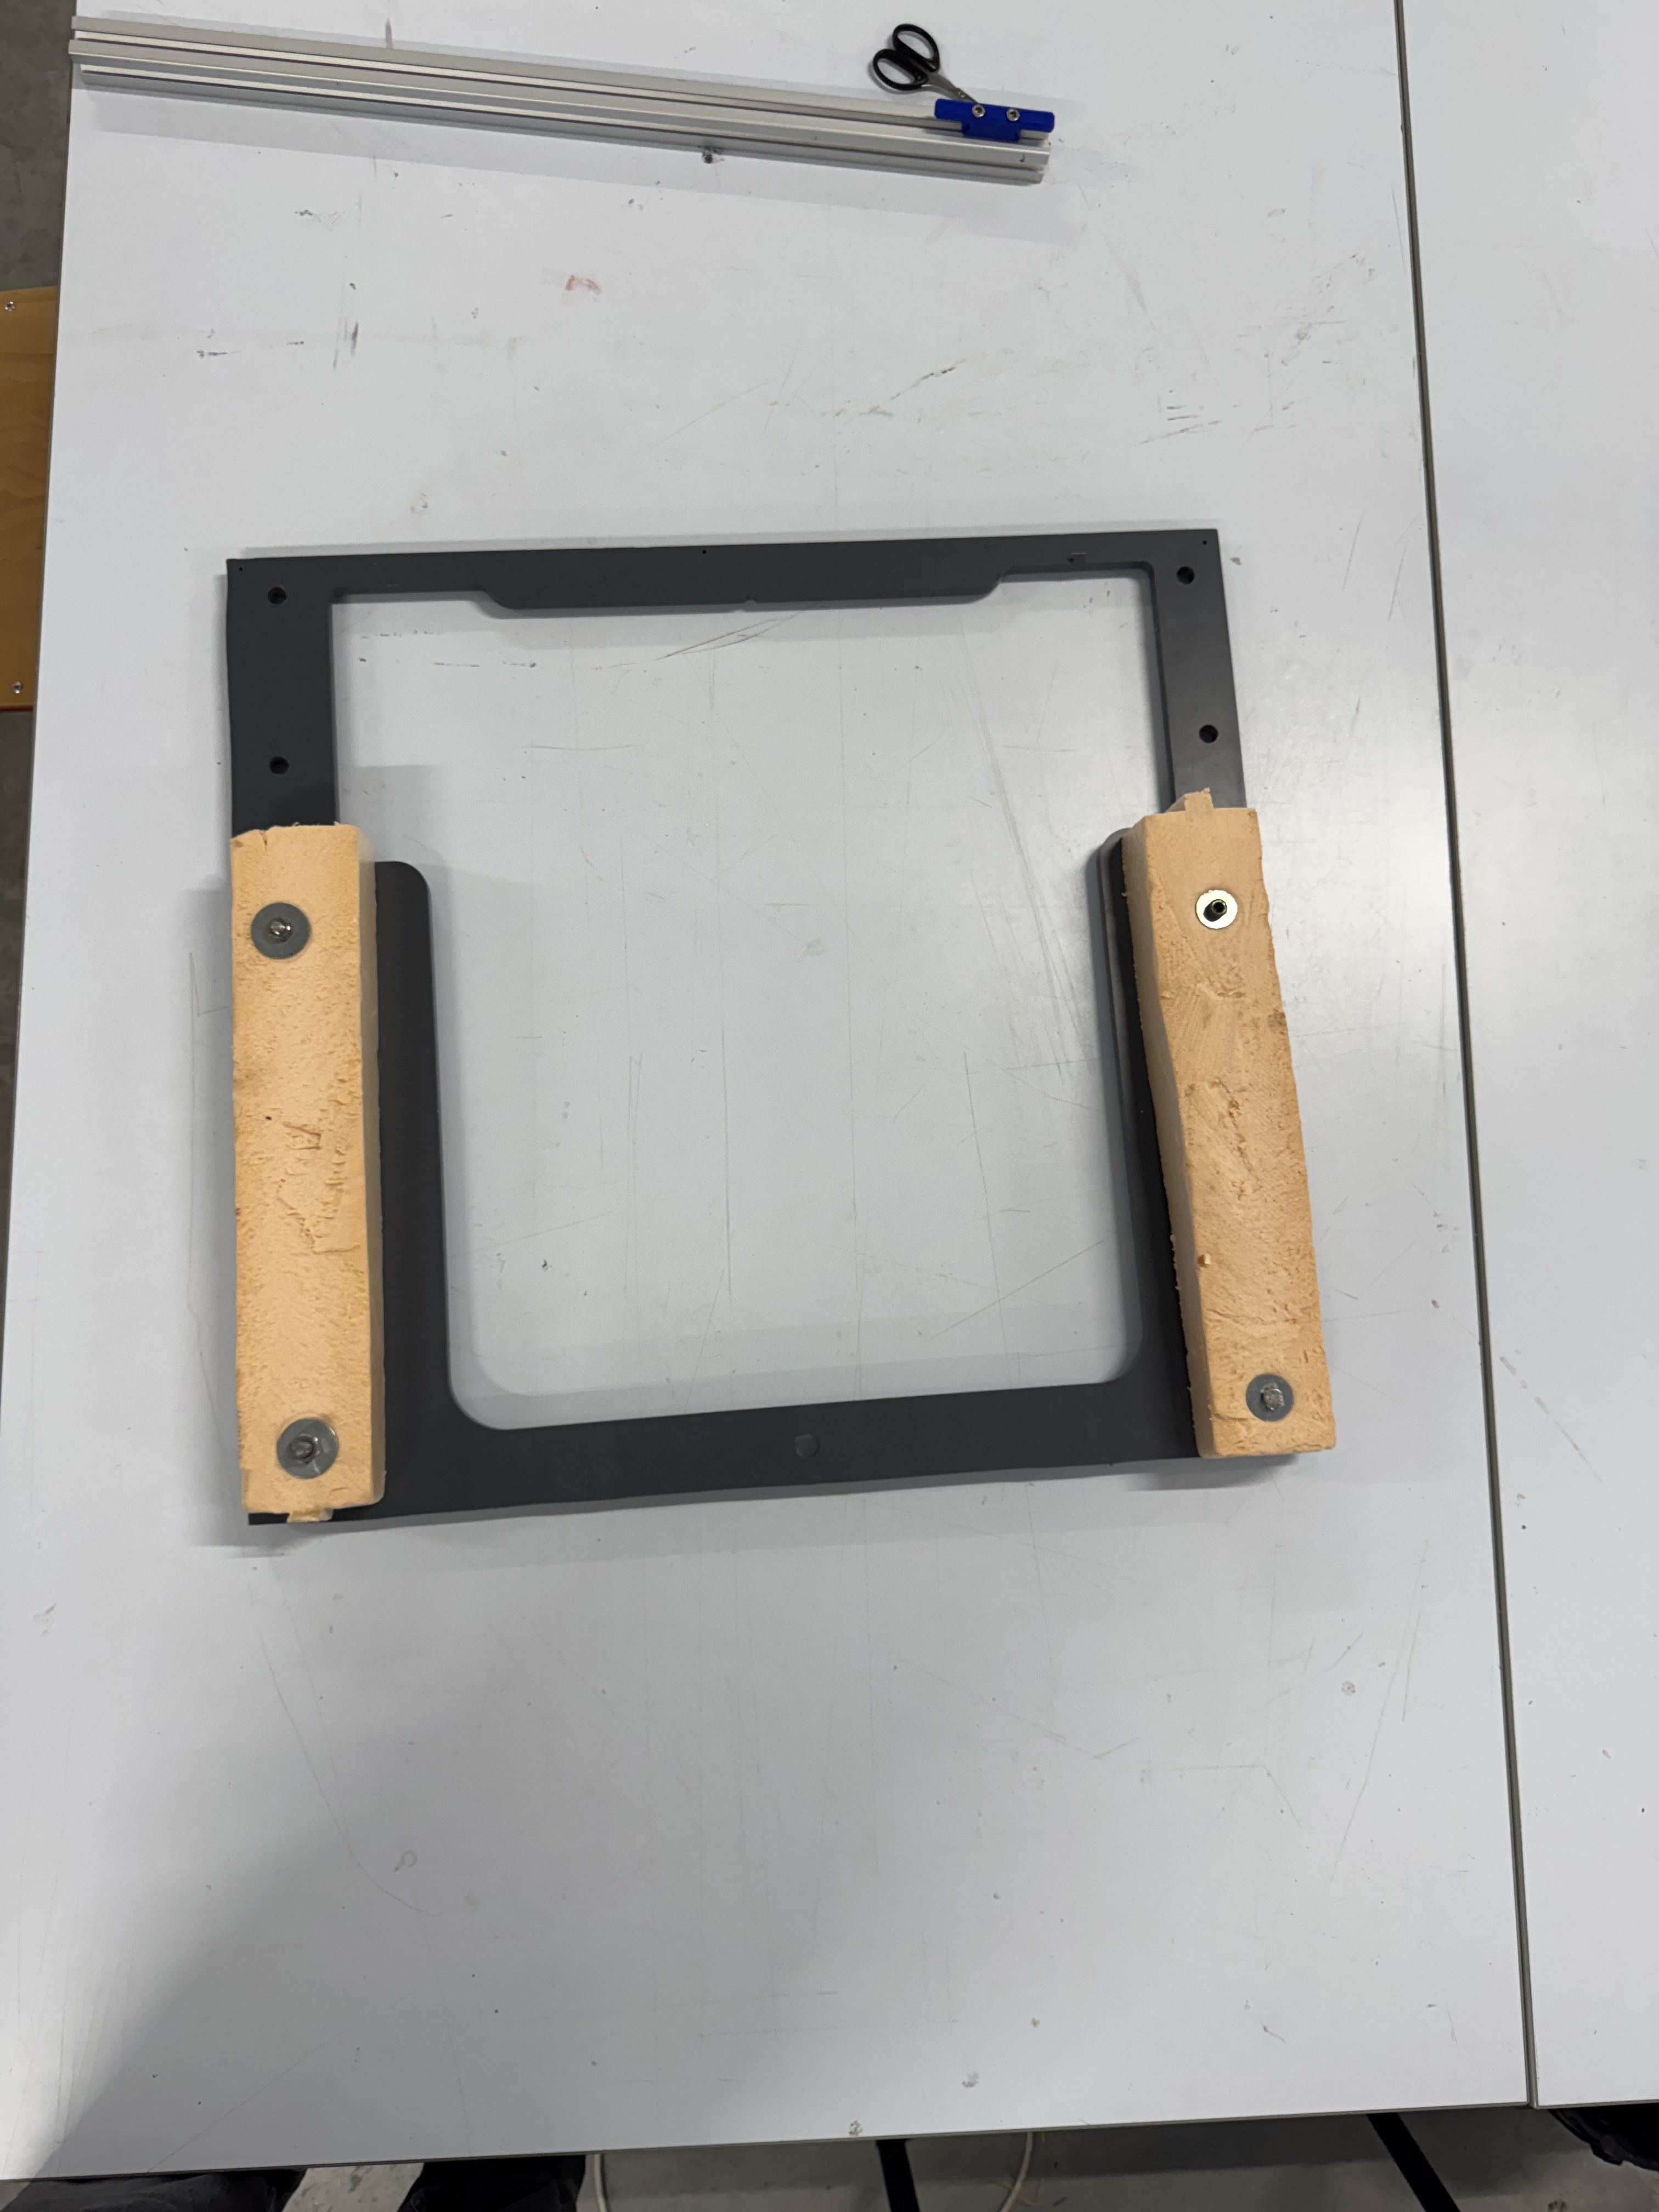
\includegraphics[width=0.6\textwidth]{images/Cage.png}
    \caption{Prototype initial : structure simple en PVC représentant l'entrée de la cage}
    \label{fig:cage}
\end{figure}

\subsubsection*{Phase d'expérimentation : évaluation de différents réflecteurs}

Afin d'améliorer la visibilité acoustique, une série de tests comparatifs a été réalisée en lac avec différents matériaux réfléchissants fixés sur les montants verticaux. Les candidats évalués (figure~\ref{fig:support_cage}) incluaient :

\begin{figure}[H]
    \centering
    \includegraphics[width=0.8\textwidth]{images/mousses.jpg}
    \caption{Panoplie des supports réfléchissants testés : bouées en mousse, pare-battages, petites bouées en plastique}
    \label{fig:support_cage}
\end{figure}

\begin{itemize}
    \item Bouées en mousse : signature acoustique intense mais géométrie irrégulière.
    \item Pare-battages : échos stables mais surface réfléchissante limitée.
    \item Petites bouées blanches : faible contraste acoustique à moyenne portée.
\end{itemize}

La figure~\ref{fig:supports_cage_tous} présente les images sonar correspondantes. Ces essais ont révélé que la géométrie et l'orientation des réflecteurs influencent fortement la stabilité de la détection. Aucun de ces supports isolés ne garantissait une signature robuste sur toute la plage d'approche (1--15 m).

\begin{figure}[H]
    \centering
    % --- Première image ---
    \begin{subfigure}[b]{0.32\textwidth}
        \centering
        \includegraphics[width=\textwidth]{images/mousses_oranges.png}
        \caption{Bouées en mousses}
        \label{fig:mousse_a}
    \end{subfigure}
    % --- Deuxième image ---
    \begin{subfigure}[b]{0.32\textwidth}
        \centering
        \includegraphics[width=\textwidth]{images/parbates.png}
        \caption{Pare-battages}
        \label{fig:mousse_b}
    \end{subfigure}
    % --- Troisième image ---
    \begin{subfigure}[b]{0.32\textwidth}
        \centering
        \includegraphics[width=\textwidth]{images/ptites_bouees_blanches.png}
        \caption{Petites bouées en plastique}
        \label{fig:mousse_c}
    \end{subfigure}

    % Légende globale et label global
    \caption{Comparaison des signatures acoustiques obtenues en lac avec différents réflecteurs}
    \label{fig:supports_cage_tous}
\end{figure}

\subsubsection*{Configuration finale : cage cubique avec cordages et panneaux absorbants}

Suite à ces expérimentations, la configuration retenue combine une structure cubique en profilés aluminium permettant l'entrée complète du véhicule et son maintien lors des manœuvres de relevage. La cage est équipée :
\begin{itemize}
    \item d'enroulements de cordages sur trois faces, générant des échos intenses et une signature acoustique riche,
    \item de plaques de PVC intégrées aux enroulements pour atténuer les réflexions parasites du grillage métallique de fond.
\end{itemize}

Cette solution exploite les propriétés complémentaires des matériaux testés : réflectivité élevée des cordages et absorption ciblée des panneaux de PVC.

\begin{figure}[H]
    \centering
    \includegraphics[width=0.6\textwidth]{images/cage_cubique.JPEG}
    \caption{Cage cubique finale en cours d'assemblage, équipée de cordages réfléchissants et panneaux absorbants}
    \label{fig:cage_cubique}
\end{figure}

\begin{figure}[H]
    \centering
    \includegraphics[width=0.7\textwidth]{images/cage_pvc_cordes.JPEG}
    \caption{Vue détaillée de la cage avec panneaux de PVC et enroulements de cordages}
    \label{fig:cage_pvc_cordes}
\end{figure}

\begin{figure}[H]
    \centering
    \includegraphics[width=0.7\textwidth]{images/sonar_cage_piscine.png}
    \caption{Image sonar de la cage finale en bassin : signature acoustique stable et géométrie exploitable (image brut à gauche, image traitée à droite)}
    \label{fig:sonar_cage_finale}
\end{figure}

La figure~\ref{fig:sonar_cage_finale} confirme que cette configuration produit une signature exploitable par l'algorithme de traitement d'image décrit en Partie~I. Le grillage métallique génère des échos caractéristiques à profondeur fixe, tandis que les cordages assurent la détectabilité à différentes portées. Cette solution garantit une perception robuste dans toutes les phases du docking.

\subsection{Contrôle du robot}

Le contrôle du BlueROV Heavy s'effectue via une manette de jeu (fig.~\ref{fig:manette_annexe}) permettant à l'opérateur de commander manuellement les six degrés de liberté du véhicule ou d'activer des modes automatiques (maintien de profondeur et de cap par régulateurs PID). Les détails complets de l'utilisation de la manette sont fournis en Annexe~\ref{appendix:controle-bluerov}.

\section{Validation Expérimentale du Système de Docking}

Après la phase de conception matérielle décrite précédemment, le système complet (algorithmes de traitement d'image, contrôleurs de navigation, cage optimisée) a été validé expérimentalement dans deux environnements distincts : un bassin contrôlé puis un lac en conditions réelles.

\subsection{Essais en Bassin ENSTA}

Les premiers essais de validation du système complet de docking ont été réalisés dans le bassin de l'ENSTA Bretagne. L'objectif principal de cette phase était de confirmer la détection de la cage et la réussite du suivi par tracker dans un environnement contrôlé. 

Le bassin, de par sa taille limitée, présente une caractéristique intéressante pour la validation : les parois et le fond génèrent de multiples échos parasites qui se superposent à la signature acoustique de la cage. Ces réflexions multiples constituent un environnement acoustique particulièrement bruité, bien plus complexe que celui rencontré en lac où l'espace ouvert atténue naturellement ces phénomènes de réverbération. La capacité du système à détecter et suivre la cage dans ces conditions difficiles représentait donc un test exigeant, garantissant que les algorithmes de traitement d'image et le tracker CSRT fonctionneraient de manière robuste lors des essais ultérieurs en environnement réel.

\textit{[Instruction : Ajoutez les dimensions du bassin (longueur, largeur, profondeur). Précisez la configuration de la cage (fixée au fond ou suspendue). Décrivez le protocole : position de départ du ROV, procédure de lancement de l'autonomie, critères de succès (positionnement à 1m de la cage avec alignement correct). Mentionnez les outils de vérité terrain utilisés si disponibles (caméras externes, système de localisation).]}

\subsection{Campagne d'Essais : Lac de Guerlédan}

Afin de valider la robustesse du système en conditions réelles, une campagne a été menée au lac de Guerlédan.

\textit{[Instruction : Décrivez les conditions environnementales spécifiques : turbidité de l'eau (visibilité réduite), présence potentielle de courants, profondeur d'opération. Expliquez les défis logistiques (mise à l'eau depuis un ponton ou un bateau). Comparez la signature acoustique de la cage dans cet environnement "bruité" par rapport au bassin (réverbération du fond, objets parasites).]}

\subsection{Analyse des Résultats Expérimentaux}

Cette section synthétise les données collectées lors des deux campagnes d'essais.

\textit{[Instruction : Comparez les trajectoires réelles du ROV avec celles de la simulation. Présentez des statistiques de réussite (ex: "Sur 20 tentatives, 15 ont abouti à un amarrage réussi"). Analysez les échecs : est-ce un problème de perte de la cible au sonar (perception) ou une incapacité des propulseurs à contrer une perturbation (commande) ? Incluez des images sonar réelles montrant la cage vue par le robot à différentes distances.]}




